    %\subsubsection{VR integration and data visualization interface}
    %\label{subsubsec:VR_integration}
    %%Define the sections of the VR interface and how information is displayed
    %\input{Text/VR_integration}


The final component of the VR system is the `Virtual reality integration' module, which serves as the bridge between the virtual environment generated by the `3D modeling' component and the data derived from the complexity analysis of facade variations, provided by the CICA system.
This integration culminates in an immersive virtual reality application developed using Unity (v.2022.2.21f1), accessible through a Head-Mounted Display (HMD) like the Oculus Quest 2.


This module includes an immersive simulation and a data visualization interface that transports users into the VR simulation of the experiment's location for facade complexity analysis.

Within this dynamic virtual environment, participants can explore and interact with the building from both inside and outside, visualize its context, and manipulate the facade variations through the user interface.

Seamlessly integrated with the simulation, the interface provides real-time feedback on the impact of different facade variations on the building, facilitating more effective and informed decision-making when selecting a specific level of complexity.

%%% Figure of Real building next to VR
     \begin{figure}[htb]
          \centering
          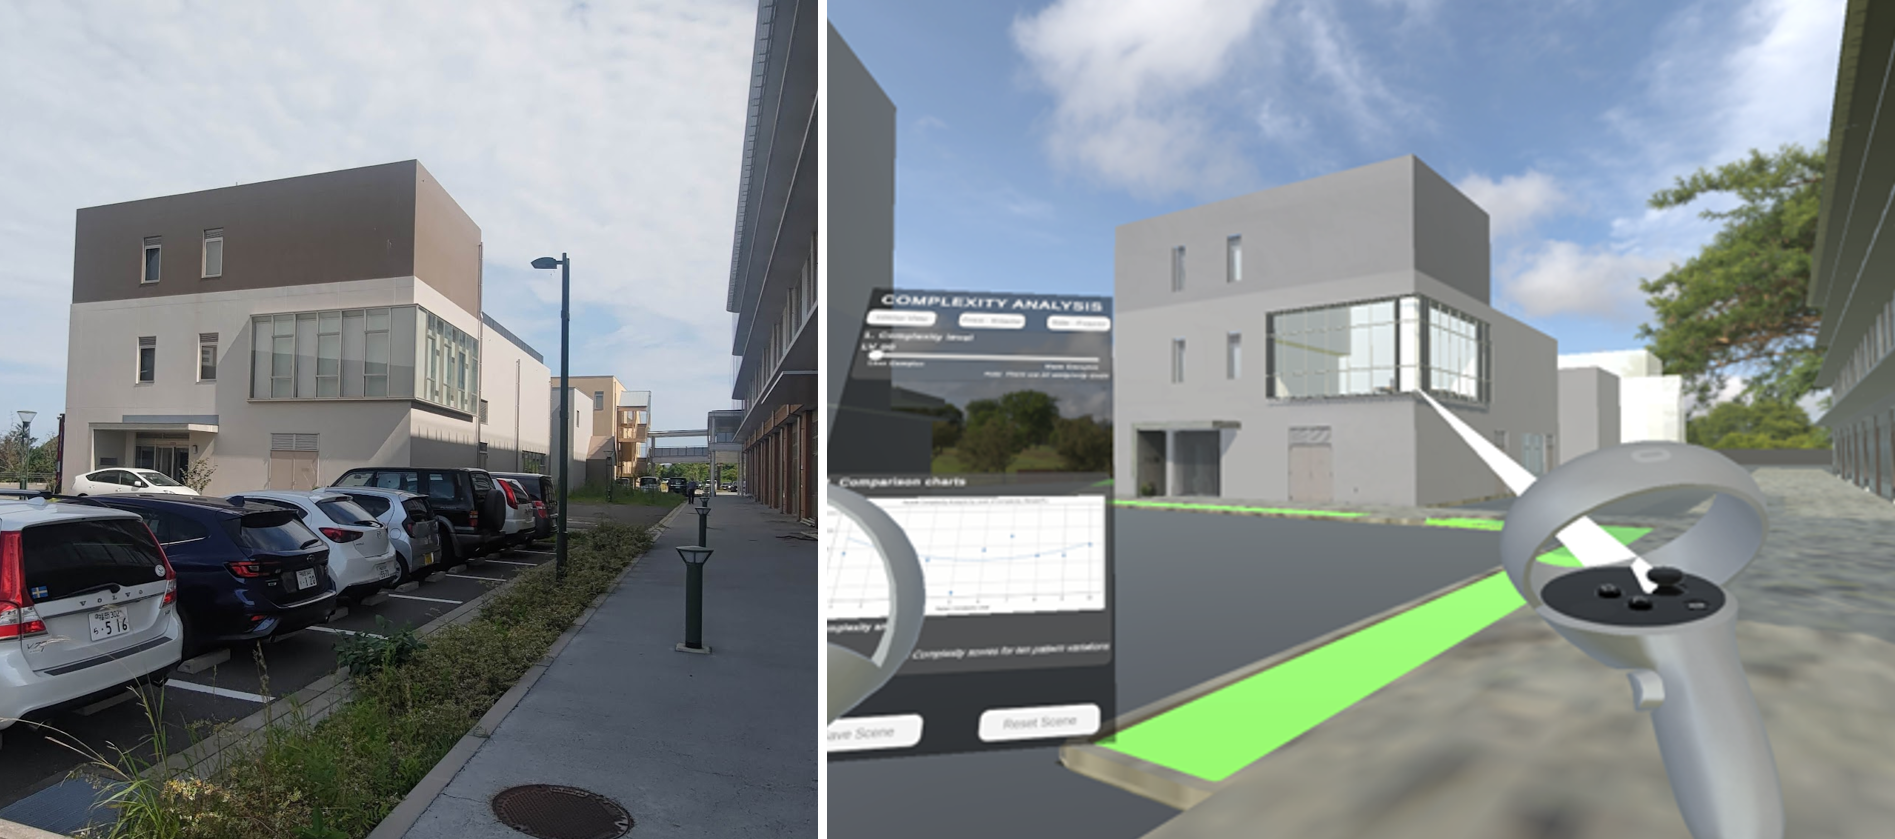
\includegraphics[width= \linewidth]{Images/RealvsVRBuildling}
          \caption{Comparison side by side of actual photography (left) of laboratory building used for experiment and virtual clone (right) modeled and simulated in VR for the Complexity analysis experiment in facade design.}
          \label{fig:RealVsVR}
        \end{figure}

%% Figure of interior and exterior VR
     \begin{figure}[htb]
          \centering
          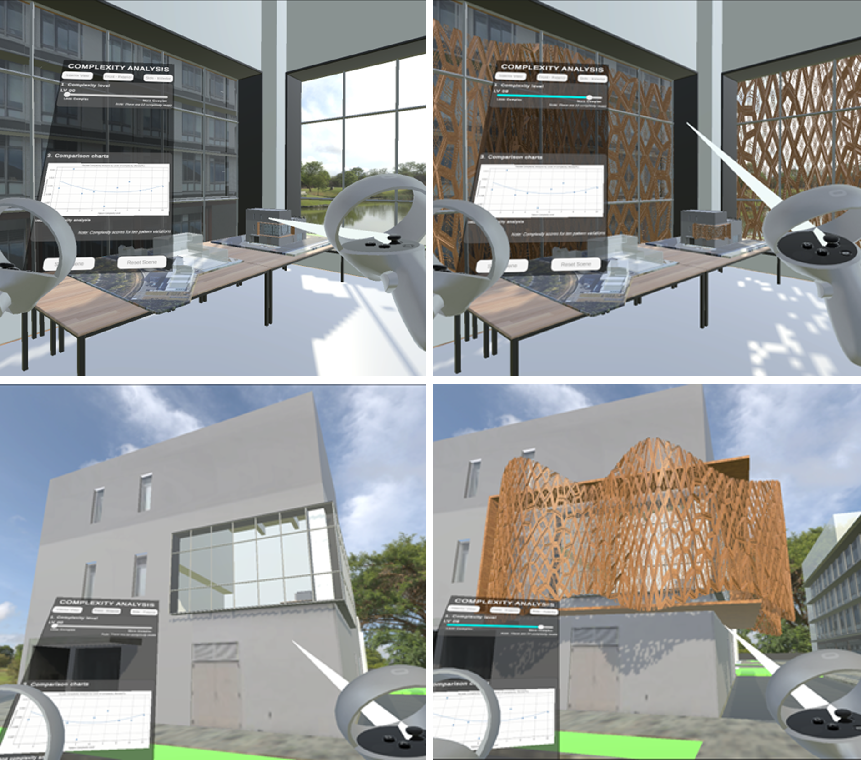
\includegraphics[width= \linewidth]{Images/VRInteriorExterior}
          \caption{VR simulation of interior and exterior of existing building at Kyushu University. (Left) Simulation of current building and (Right) simulation of Complex façade variation.}
          \label{fig:VRInteriorExterior}
        \end{figure}

%!Vr interface

The VR data visualization interface, as illustrated in Figure\ref{fig:VRInterface}, is designed with four key sections to enhance the usability and interpretability of the transition between facade variations.

%% Figure of interface VR
     \begin{figure}[!htb]
          \centering
          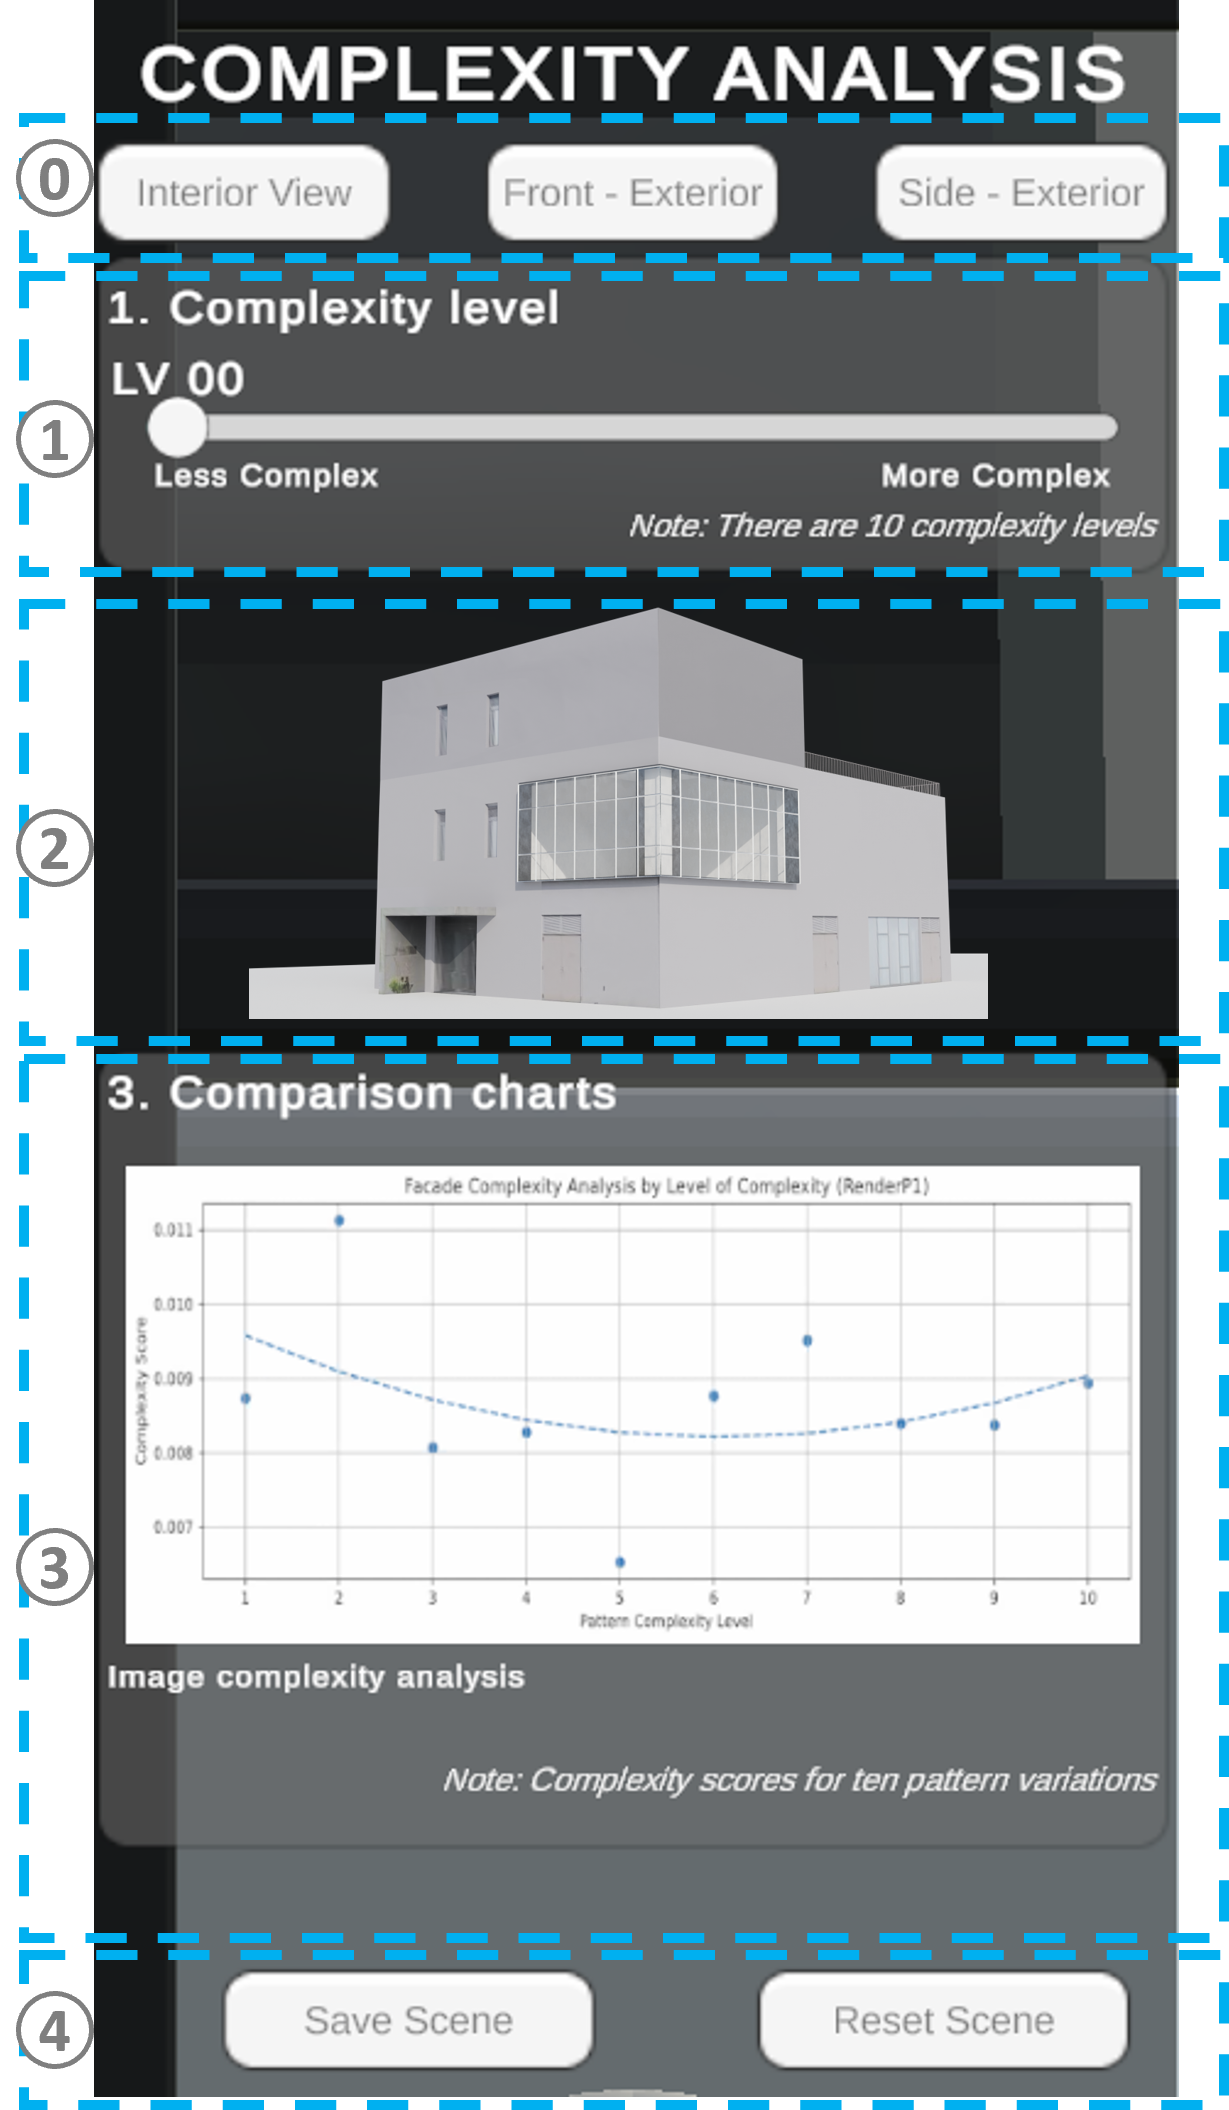
\includegraphics[width= \linewidth]{Images/VRInterface}
          \caption{VR interface for complexity tolerance analysis in facade design. 0) Predetermined cameras, 1) Slider with ranking of levels of complexity, 2) Render preview of facade design, 3) Comparison scatter graph with complexity scores per level of complexity, 4) Save and reset buttons also used to transition among the three patterns.}
          \label{fig:VRInterface}
        \end{figure}

At the top, three buttons offer predetermined camera views, enabling users to examine the facade variations from the inside of the lab and from the outside of the building.
Just below, a slider displays the 10 facade variations ranked in accordance with its complexity score in addition of a `level 0' representing the initial or current stage of the actual building for reference.

This slider is linked to the facade allowing the user to exchange the building envelop and select the one they feel the most comfortable with among the ten variations.
The facade is simultaneously changed on the building and in a scaled model of the building simulated inside the lab so that the user of the application can experience the impact of the facade from inside the lab while simultaneously having feedback of the building exterior on the scale model as depicted in Figure\ref{fig:VRInteriorExterior}.

Bellow the slider there is an image preview with a photo-realistic render of the building as seen from the outside.
This helps to retain a constant feedback of the impact of the facade in the building specially useful when exploring the simulated interior of the lab.

In the following section, labeled `3) Comparison charts', the scatter graph depicts the individual scores of each facade variation determined for a specific pattern in accordance with the Computational Image Complexity Analysis (CICA) system.
This feature ensures users have access to  a data visualization tool to inform them of the selection process used for ranking the facade variations in hopes of facilitating the decision-making process when selecting a facade variation.

Finally, at the bottom of the interface, two buttons are available.
One button allows users to reset the application, providing a fresh start if needed.
The other button allows users to save the selected facade variation for the building, preserving their selection per pattern and to save it to our database to evaluate the results.

Overall, the VR integration interface serves as an interactive tool for effectively measuring the user response to varying levels of complex facades in an intuitive and dynamic manner, it empowers designers to explore in a real world scale the implications that a facade has on the perception of a built space, making the decision-making process of selecting a specific level of complexity more efficient and informed.






